\section{Why and what}
By the strict point of view of the cost of software development we can say that software re-use reduces the cost so it is better to buy off-the-shelf products and components than re-implementing them.
Moreover since we have moved from software product to product families it is always more and more important to build flexible products and construct systems by composing components is easier.
Also it is more reliable to re-use software than to create new one and some use case force the use of certified components then the emergence of distributed and concurrent systems tells us the necessity to build systems composed of independent parts.

Software components should be in software engineering like integrated circuits in electronic engineering, just like lego blocks:
\begin{itemize}
    \item \emph{modular}: a component should be self-contained, should expose a simple interface to achieve \emph{compatibility}, should serve various purpose in order to exploit \emph{re-usability} and, of course should be the base for bigger components, so it should be \emph{extensible};
    
    \item \emph{reliable}: it should do what it's supposed to do according to the specifics, so it must be \emph{correct} and \emph{robust} in order to achieve it's scope in abnormal conditions;
    
    \item \emph{efficient};
    \item \emph{portable}: should be transferable between different platforms;
    \item \emph{timely}: released when or before users want it.
\end{itemize}

\subsection{Definition}
A definition of software component is the following according to Clemens Szyperski: \emph{a software component is a unit of composition with contractually specified interfaces and explicit context dependencies only.
A software component can be deployed independently and is subject to composition by third parties.}

\subsubsection{Composition unit}
A composition unit is a black box of which you don't necessarily have the source code, it's partial deployment is not possible.
A system is built combining those components with some glue code and each component has no externally observable state and is indistinguishable from other copies.

\subsubsection{Contract}
A component must expose an interface that implements a contract which is the group of specifications of functional aspects (the API), the pre and post conditions for the operations specified by the APIs and the non functional aspects which are for example the constraints or the environment requirements.
Moreover a contract also specifies how the component can be deployed, how can be instantiated and how the instances act through the public interfaces.

Of course there is the need of an Interface Definition Language in order to have coherent specifications across the various components.

\subsubsection{Explicit context dependency}
The component need to specify the deployment environment and the run-time environment, for example which tools, platforms, resources or other components are required for the correct functioning.

\subsubsection{Deployed independently}
The components are all hosted on a platform (framework in later concepts) which orchestrates them.
The dependencies are resolved at load or at run-time exploiting the \emph{late binding} and sometimes need the use of a \emph{connector} to adapt the provided interfaces.

\subsection{Component model}
The basic concepts of a component model are:
\begin{itemize}
    \item component interface: is the description of the operations that a component implements and that other component may use, for example is the list of method calls, the message format, the endpoints list;

    \item composition mechanism: the manner in which different components can be composed to work together.
    
    \item component platform: the platform for the development and the execution of the components (the framework for which the components are developed).
\end{itemize}
Those concepts are language and paradigm agnostic and components too can be developed using different technologies in order to build language interoperability.

\subsection{Modules}
The support for some kind of modules exists in languages from 70's and is one of the main feature that enables the development of large applications providing information hiding by the encapsulation of functionalities behind a black box interface and also reduces the risks of name conflicts because it enables to import just a subset of the module.
Moreover teams can work on separate modules in a project.

Modules encapsulate variables, data type and subroutines in a package:
\begin{itemize}
    \item entities inside the package are visible one to another;
    \item entities inside are not visible outside unless explicitly exported;
    \item entities outside can be:
    \begin{itemize}
        \item visible: we refer as open scope;
        \item not visible unless imported: we refer as closed scopes;
        \item visible using a qualified name (usually via dot notation traversing the package): we refer as selectively open scopes.
    \end{itemize}
\end{itemize}
So the module interface specifies the exported entities but the module is compiled separately and implementation details are hidden to outside of the module.

\subsubsection{Some implementations}
Basically a module is a collection of data with some operations defined on them (basically an abstract data type).
Some implementations of this concept are:
\begin{itemize}
    \item modules as manager: we specify the instance on which to operate as additional arguments to subroutines;
    \item modules as types;
    \item object oriented way: the module is the class and you instantiate instances and call routines on them.
    It is important to notice that many object oriented languages support module independently from classes, in that case the module take the name of package.
\end{itemize}

\subsection{OOP vs COP}
The primary concern of OOP is domain and problem representation not code reuse, that's because experience has shown that the use of object oriented does not necessarily produce reusable software.

\section{Component Based Software Engineering}
This software engineering approach provides methodologies and tools for:
\begin{itemize}
    \item build systems from components;
    \item build components as reusable units;
    \item perform maintenance by replacement of components and introducing new components into the system;
    \item architect systems in terms of components.
\end{itemize}

\subsection{Component forms}
\subsubsection{Component specification}
Is the specification of a unit of software that describes the behaviour of a set of component objects and defines a unit of implementation.
The behaviour is defined as a set of interfaces and a specification is realized with an implementation.

\subsubsection{Component interface}
Is the definition of the set of behaviours that the component object offers.

\subsubsection{Component implementation}
Is the actual realization of the specification and is independently deployable, so it can be installed and replaced independently of the other components.
Of course it can have some dependencies in the other components and not necessarily is a single physical item.

\subsubsection{Installed component}
Is an installed (deployed) copy of the implementation.
A deploy is done by registering it with the runtime environment (the orchestrating framework) so that the runtime can use it during it's job.

\subsubsection{Component object}
Is an instance of the installed component and it's a concept proper of the runtime.
An installed component can have multiple component objects (which require explicit identification) or a single one (which may be implicit).

\subsection{Definition}
The basis of CBSE is the component.
Components can be assembled according to the rules specified by the component model.
Components are assembled through their interfaces in order to build larger components or applications, this procedure is called component composition.
Component are performing in the context of a component framework and all parts conform to the component model.
In the end a component technology is a concrete implementation of a component model.

\begin{figure}[H]
    \centering
    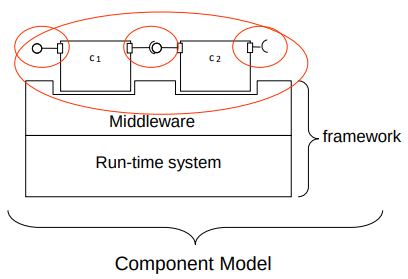
\includegraphics[width=300px]{images/3_Software_Components/component_model.png}
\end{figure}

\section{Examples}
\subsection{Old one}
The Fortran library NAGLIB which provides mathematical and physical functions is an example of successful components.
It has well defined theory behind the functions, very well standardized in the mathematical language.
It has simple interfaces in procedural style using the function call to request services.
It has well defined input and output, relative good error handling but is not so flexible.

\subsection{Big one}
\subsubsection{Database servers}
Both relational databases and NoSQL one.
The standard APIs are the SQL language or the json based language used for the interaction.

\subsubsection{X-windows}
Is the most used graphic server in Linux environment, it provides standard APIs exploiting the callback type of communication.
It has high level of adaptation but it's too general for the various use cases and so is difficult to use.

\subsection{Operating systems}
For example UNIX is a general purpose OS who exposes standard API according to POSIX.
It provides also low-level but well-defined interfaces.
Since there are more operating systems there are also different APIs not adherent to POSIX so in reality the operating system is not a real component because it is difficult to replace or update.

\subsection{More recent}
Some of the modern examples are:
\begin{itemize}
    \item plugin architecture: for finer-grained components.
    Some implementations are in the netscape's navigator web browser, in the Active Server Pages (ASP) or Java Server Pages (JSP);
    \item Microsoft's Visual Basic;
    \item Java Beans and Enterprise JavaBeans;
    \item Microsoft's COM+;
    \item android's component based apps;
    \item application and integration servers around J2EE and .NET.
\end{itemize}

\subsection{Common things}
In all the example provided there is an infrastructure providing rich foundational functionality for the scope.
Components can be purchased from independent providers and deployed by clients.
The components are big and well enough to make the development of a new variant too difficult or not cost-effective.

\section{JavaBeans}
JavaBeans API born in 1996 as an attempt to define a software component model for Java, allowing vendors to create and ship Java components that can be composed together into applications by end users.
The design goals were:
\begin{itemize}
    \item granularity: from small to medium components (a button, a window or a full spreadsheet);
    \item portability: which is by design in java based application and enlarged to other component model with some bridges;
    \item uniformity and simplicity: the API should be simple in order to be largely supported.
\end{itemize}

By definition: \emph{a Java Bean is a reusable software component that can be manipulated visually in a builder tool}.
Those components can be used to build web pages, visual applications, GUI layout or server applications.

A bean typically has a GUI representation but there exists invisible beans too and any java class can be recognized as a bean in a tool provided that:
\begin{itemize}
    \item it has a public default constructor (with no arguments);
    \item it implements the interface \verb|java.io.Serializable|;
    \item it is in a \verb|jar| file with the manifest file containing \verb|Java-Bean: True|.
\end{itemize}

\subsection{Common features}
\begin{itemize}
    \item properties: both for customization and for programmatic use;
    \item events: communication metaphor that can be used to connect several beans;
    \item customization: inside the builder tool the user can customize the appearance and behaviour of the bean;
    \item persistence: a customization can be saved away and reloaded later on;
    \item introspection: a builder tool can analyze how the bean works exploiting reflection Java APIs.
\end{itemize}

\subsection{Properties}
Properties are discrete named attributes that can affect a bean instance's appearance or behaviour.
A property can be determined and modified using the public getter and setter methods and can be changed at design time or run-time.
For example in the case of a \verb|background| property we could have:
\begin{verbatim}
public java.awt.Color getBackground();
public void setBackground(java.awt.Color color);
\end{verbatim}

\subsection{Introspection}
Introspection is the process of analyzing a bean to determine the public interface that the builder tool can present to the user.
It can be done:
\begin{itemize}
    \item implicitly: which is based on reflection, naming convention and some design patterns;
    \item explicitly: using a \verb|<BeanName>BeanInfo| class to explicitly describe info about a bean.
\end{itemize}

\subsubsection{BeanInfo class}
Using a custom BeanInfo class it is possible to only expose the feature we want the bean to expose (and rely on reflection for exposing some other ones), we can associate an icon with the target bean, specify a \verb|customizer| class, segregate features into normal and expert categories and provide additional information about the single features, like a docs would do.

\subsection{Simple properties}
Some common patterns for simple properties are the usage of the following method signatures for getter/setter:
\begin{verbatim}
    public <PropertyType> get<PropertyName>();
    public void set<PropertyName>(<PropertyType> a);
\end{verbatim}
which automatically infers the existance of a property \verb|PropertyName| with the type \verb|PropertyType|.

NB: if only the getter method is present then the property is read-only while if it only exists a setter then the property is write-only.

Another common approach if a property is an array is to specify the index during the access:
\begin{verbatim}
    public java.awt.Color getSpectrum (int index);
    public java.awt.Color[] getSpectrum ();
    public void setSpectrum (int index, java.awt.Color color);
    public void setSpectrum (java.awt.Color[] colors);
\end{verbatim}

\subsubsection{Bound property}
A bound property generates an event when the property is changed.

\subsubsection{Constrained property}
A constrained property can only change value if none of the registered observers \emph{poses a veto}.

\subsection{Connection oriented programming}
Is a paradigm used to glue together components in a builder tool.
It's based on the \emph{observer} design pattern and is pretty useful for GUIs.

\subsubsection{Observer design pattern (Publish-Subscribe)}
It's a behavioral pattern which is used during the definition of a one-to-many dependency among objects so that when one object changes state, all of its dependents are notified and updated automatically.

\begin{figure}[H]
    \centering
    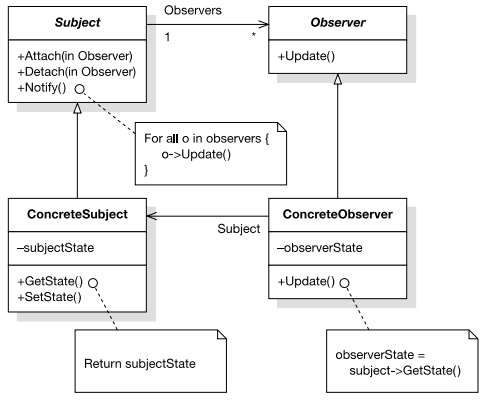
\includegraphics[width=300px]{images/3_Software_Components/Observer_pattern_UML.png}
    \caption{Observer design pattern UML diagram}
\end{figure}

\subsection{Events}
In Java the observer pattern is based on Events and Event listeners.
An \emph{event} is an object created by an \emph{event source} and propagated to the registered \emph{event listeners}.

It's multicast by design because multiple listeners can register for the same event but of course it can be restricted to unicast.

There is a common naming convention for the event source:
\begin{verbatim}
    public void add<EventType>Listener(<EventListType> a)
    public void remove<EventType>Listener(<EventListType> a) 
\end{verbatim}

NB: unicast sematics is assumed if the add listener method is declared to throw \\
\verb|java.util.TooManyListenerException|.

Events are used in the implementation of bound properties.
The event used is of type \\
\verb|PropertyChangeEvent| and is sent to objects that previously registered an interest in receiving such notifications.

\subsubsection{Event adaptors}
Is placed between an event source and an event listener.
It's a listener and a source at the same time.
Some usage of an adaptors are:
\begin{itemize}
    \item implement an event queue;
    \item act as a filter;
    \item aggregate multiple event source into a single event listener;
    \item generic wiring manager between sources and listeners.
\end{itemize}

\subsubsection{Implement Bound Property in a Bean}
\begin{itemize}
    \item import \verb|java.beans| package;

    \item instantiate a \verb|PropertyChangeSupport| helper object:
    \begin{verbatim}
private PropertyChangeSupport changes = new 
    PropertyChangeSupport(this);
    \end{verbatim}

    \item implement methods to maintain the property change listener list:
    \begin{verbatim}
public void addPropertyChangeListener(PropertyChangeListener l){
    changes.addPropertyChangeListener(l);
}
    \end{verbatim}
    and \verb|removePropertyChangeListener|
    
    \item fire the event when the property setter method is called:
    \begin{verbatim}
public void setX(int newX){
    int oldx = x;
    this.x = newX;
    
    changes.firePropertyChange("x", oldX, newX);
}
    \end{verbatim}
\end{itemize}

\subsubsection{Implement a Bound Property Listener}
\begin{itemize}
    \item the listener beam must implement the interface \verb|PropertyChangeListener|:
    \begin{verbatim}
public class MyListener implements PropertyChangeListener,
    Serializable{
...
}
    \end{verbatim}

    \item it must override the method \verb|propertyChange|:
    \begin{verbatim}
public abstract void propertyChange(PropertyChangeEvent evt){
...
}
    \end{verbatim}
\end{itemize}

\subsubsection{Implement Constrained Property in a Bean}
\begin{itemize}
    \item import the \verb|java.beans| package;

    \item instantiate a \verb|VetoableChangeSupport| object:
    \begin{verbatim}
private VetoableChangeSupport vetos = new 
    VetoableChangeSupport(this);
    \end{verbatim}

    \item implement methods to maintain the listener list:
    \begin{verbatim}
public void addVetoableChangeListener(VetoableChangeListener l){
    vetos.addVetoableChangeListener(l);
}
    \end{verbatim}
    and \verb|removeVetoableChangeListener|

    \item write a property's setter method to fire a propery change event:
    \begin{verbatim}
public void setX(int newX){
    int oldX = this.X;
    
    try{
        vetos.fireVetoableChange("X", oldX, newX);
        // here only if no veto
        this.X = newX;
        // notify change if needed
    }
    catch(PropertyVetoException e){
        // code if change is rejected by somebody
    }
}
    \end{verbatim}
\end{itemize}

\subsubsection{Implement a Constrained Property Listener}
\begin{itemize}
    \item the listener beam must implement the interface \verb|VetoableChangeListener|:
    \begin{verbatim}
public class MyListener implements VetoableChangeListener,
    Serializable{
...
}
    \end{verbatim}
    
    \item it must override the method \verb|vetoableChange|:
    \begin{verbatim}
public void vetoableChange(PropertyChangeEvent evt){
...
}
    \end{verbatim}
    this is the method that will be called by the source bean on each listener registered to the source;
    
    \item if the listener wants to forbid the change described in the event it should raise a \\
    \verb|PropertyVetoException| otherwise simply terminate the method.
\end{itemize}

\section{The Microsoft way}
The Microsoft approach passes by continuous re-engineering of existing applications, the component technology has been introduced gradually taking advantage of previous success (Visual Basic controls, Active X, ASP) ad using reviews from main older approach (the COM - Component Object Model) to build current .NET + CLR.

\subsection{Component Object Model}
It was the MS component technology before .NET, has been made available on other platforms with little success.
This model doesn't prescribe language, structure or implementation of an application, it just specifies an object model and programming requirements that enable COM components to interact, it is a \emph{binary standard for interfaces}.
The only requirements for the language is that the used language needs to create structures of pointers and, either explicitly or implicitly, call functions through pointers (so C++ for example is good but Java, C, and many other can be used as well).

A COM interface is a pointer to an interface node which is a pointer to a table of function pointers called \emph{vtable}.
When an operation of the interface is invoked a pointer to the interface itself is passed as an additional argument, just like the \emph{this} or \emph{self} pointer in some OOP languages, this pointer is used to access instance variables.

A COM component may implement any number of interfaces, all the implementation can be defined in a single class or splitted across different ones.
In the end a component can contain many object of different classes to build the functionalities.
\begin{figure}[H]
    \centering
    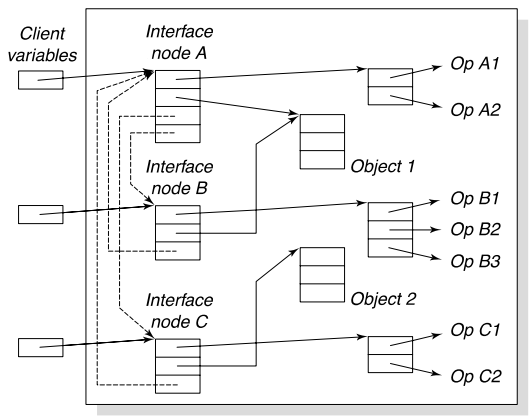
\includegraphics[width=300px]{images/3_Software_Components/COM_module.png}
    \caption{A COM object with multiple interfaces}
\end{figure}

\subsubsection{COM interface}
The identity of the interface is determined by a Globally Unique Identifier (GUID) or by a non-unique name.
The root of the interface hierarchy is \verb|IUnknown| and defines:
\begin{itemize}
    \item \verb|QueryIterface|: is a function that given a GUID returns an interface reference if the interface is implemented by the component, otherwise returns an error (invocation of this function using the GUID of IUnknown returns the same address);

    \item Addref and Release which are used for the garbage collection via the reference counting.
\end{itemize}
basically invocation of procedures on the IUnknown are used to identify of a component.

\subsubsection{Containment and Aggregation}
COM does not support inheritance for the implementation, reuse is supported through containment and aggregation:
\begin{itemize}
    \item containment: an outer object holds an exclusive reference to an inner object, so methods of the outer objects are just proxy for the methods of the inner one.
    This method can add overhead because the proxy must be done;

    \item aggregation: a reference to the interface of the inner object is passed to the client that now is free to use it.
    The outer object can't intercept, filter nor modify the invocations of the inner methods.
    This approach though breaks transparency because the client need to know how the object is made internally in order to use it.
\end{itemize}

\subsubsection{Inheritance, polymorphism and versioning}
Single inheritance among interface is possible but rarely used but due to the QueryInterface mechanism it is impossible to know if an interface has more methods.

Polymorphism is given supporting a sets of interfaces for components: in this case the type of the component is the set of GUID of its implemented interfaces and a subtype is a superset of interfaces (because it adds more to the interface that extends).

There is no support for versioning.

\subsubsection{Creating COM objects}
An application can request a COM component at runtime based on its class.
A class identifier is a globally unique identifier too called CLSID.
There is a static procedural API that creates objects: \verb|CoCreateInstance(CLASID, IID)| which exploits a registry to identify a COM server which provides factories for COM interfaces.

\subsection{.NET framework}
The .NET framework describes .NET components local and distributed ones, connections between components and deployment.
Also it describes aggregation and containment compositions, synchronous and asynchronous method invocation and delegates and event-based communication.

It has been introduced by Microsoft in 2000 and is a platform for rapid and easy build, deploy and run .NET software components.
It allows rapid development of XML web services and applications, so it is highly productive, component-based and multi-language because it adds epmhasis on interoperability.

\subsubsection{Common Language Specification (CLS)}
Is the set of guidelines that languages should follow so that they can communicate with other .NET languages, moreover it ensures type safety using type matching and high performance code execution.
It also provides an object-oriented model that supports the complete implementation of many programming languages.

\subsubsection{Base Class Library (BCL)}
It is a comprehensive, consistent, object-oriented library of prepackaged functionalities and applications.
These class library can be used to develop applications that include:
\begin{itemize}
    \item traditional CLI application;
    \item GUI applications (Windows forms);
    \item Web services (ASP.NET).
\end{itemize}

\subsubsection{Common Language Runtime (CLR)}
It ensures a common runtime environment for all the .NET languages, uses a common type system (strict type and code-verification) and adds garbage collection.
Moreover it adds a compiler from intermediate language (MSIL) to native and some security features.

\subsubsection{Overview}
It supports the development and deployment of desktop, window and web-based application services on both windows and other platforms through SOAP and HTTP (and even Linux with \emph{mono}, a .NET port).
.NET supports component versions and allows COM components to be reused, moreover different version can coexist without any conflict.

It has also support for distributed components by remoting channel technology, supports interoperability between COM, .NET and XML web service components.

Is available in .NET framework SDK and Visual Studio.NET IDE SDK which enables writing, building, testing, debugging and deploying .NET applications.
It supports all .NET languages such as VB.NET, VC.NET, C\# and many others.

\subsubsection{Microsoft CLI}
CLI stands for Common Language Infrastructure and is the Microsoft initiative in building a language with the same philosophy of Java.
The idea was to exploit dynamic load of JVM to implement a component based architecture like COM.

Microsoft started extending JVM in order to add interoperability with existing COM code and to support many languages but Sun (Java's owner) complained of license infringement, so Microsoft started developing its own technology.
Based on the Java experience and the main two features above they made CLI which has at the core the Common Language Runtime (CLR) which is substantially the same as JVM for Java.
\begin{figure}[H]
    \centering
    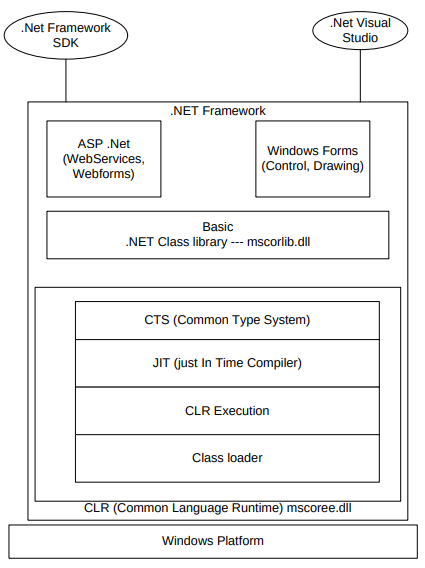
\includegraphics[width=200px]{images/3_Software_Components/CLI_infrastructure.png}
    \caption{Common Language Infrastructure}
\end{figure}

Some of the implementations are:
\begin{itemize}
    \item CLR: Microsoft's commercial offering;
    \item SSCLI (Rotor): Microsoft's shared source CLI, discontinued (free for non commercial use);
    \item Mono: open source project sponsored by Ximian and now by Microsoft.
    It adds .NET support for Linux;
    \item DotGNU portable .NET;
    \item OCL: portions of the implementation of the CLI by Intel;
    \item .Net core: open source, cross platform, supported by Microsoft and community;
    \item .Net 5.0.5
\end{itemize}

\subsubsection{Common feature with JVM}
Among the common features with JVM we have it's security, portability, Garbage collection for automatic memory management, type safety, dynamic loading, class library, OOP and mix-in inheritance.
The essential traits of the execution environment are similar but there are relevant differences in the design, moreover CLI has been standardized (by ECMA and ISO) and is a superset of Java.

\subsubsection{CLR}
Common Language Runtime is a virtual machine environment sitting on the top of the operating system.
It consists of:
\begin{itemize}
    \item Common Type System (CTS);
    \item Just-In-Time CIL compiler;
    \item Virtual Execution System;
    \item garbage collection;
    \item security management.
\end{itemize}
It is shipped in a package of assembly consisting of MS Intermediate Language (MSIL) code and manifest (metadata about the packet).
The CIL code is translated into native code by JIT compiler in CLR but only after that the CTS verifies the IL to check the validity of data type used in the code.

So the multilanguage support is given by the CLR implementation, moreover a class in one language can inherit properties and methods from related classes in other languages.
The CTS defines a standard set of data type and rules for creating new types starting from:
\begin{itemize}
    \item reference types;
    \item value types.
\end{itemize}

The code targeting CLR to be executed by it is called \emph{.NET managed code}.
All Microsoft language compilers generate managed code that conforms to the CTS.
This code is like java bytecode and can be in format of executable or dynamic link library (.dll).
Some code that is generated by non .NET compilers is called \emph{un-managed} code.
\begin{figure}[H]
    \centering
    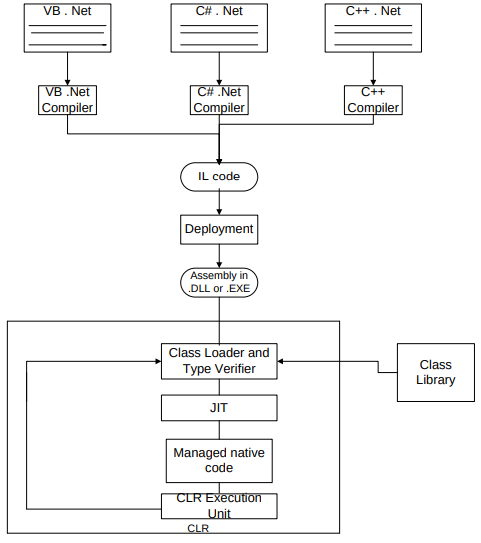
\includegraphics[width=200px]{images/3_Software_Components/CLR.png}
    \caption{CLR}
\end{figure}

\subsubsection{Common type system}
Execution environments like CLR and JVM are \emph{data oriented}, a type is the unit of code managed by the runtime so loading, code, state and permission levels are all defined in terms of types.
Applications are set of types that interact together and one type exposes a static method (\verb|Main|) which is the entry point of the application which loads the needed types and creates the appropriate instances.

The Java type system that we've already seen is far simpler than the one of CLR because to enstabish a framework to support cross-language interoperability, type safety and high performance code execution CLR defines a rich set of data types, based on an object-oriented model.
Moreover it defines rules that ensure that objects written in different languages can interact with each other, rules for scopes, type visibility and access to the member of a type.
The common language runtime enforces the visibility rules!
Moreover it defines rules of type inheritance, virtual methods and object lifetime.
Languages supported by .NET can implement only part of the common data types.

The CLR type system is hierarchically (common rooted):
\begin{figure}[H]
    \centering
    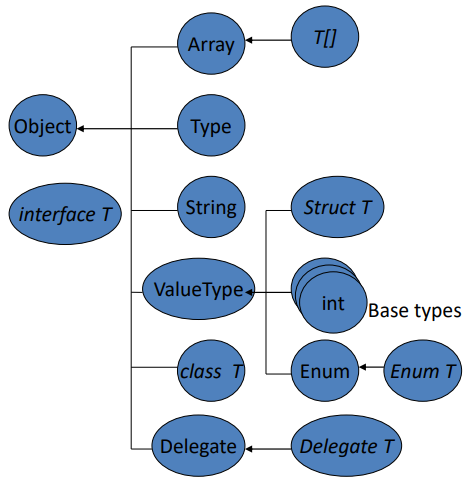
\includegraphics[width=200px]{images/3_Software_Components/common_type_system.png}
    \caption{Common type system}
\end{figure}
There are more type constructors:
\begin{itemize}
    \item \verb|Enum|: constants;
    \item \verb|Struct|: like class but with stack allocation and without inheritance;
    \item \verb|Delegate|: type that describes a set of methods with common signature.
\end{itemize}
The value types are basically numbers and structs and inherits directly from \verb|Object|, those are not reference types and aren't stored on the heap.

The trick is that when a value type should be upcasted to \verb|Object| it is \emph{boxed} in a wrapper on the heap, while the opposite operation is called \emph{unboxing}.

\subsubsection{Class library}
The .NET framework class library is a collection of reusable basic classes which are well organized by namespaces, there is a direct correspondence with Java API and Java packages.
A namespace consists of many classes and sub-namespaces and it is deployed as a component class library itself, also organized in a component-based hierarchy.
The .NET framework itself is built up in a component model and developers can create custom namespaces.
A namespace can be deployed as an assembly of binary components.

The class library is very wide:
\begin{figure}[H]
    \centering
    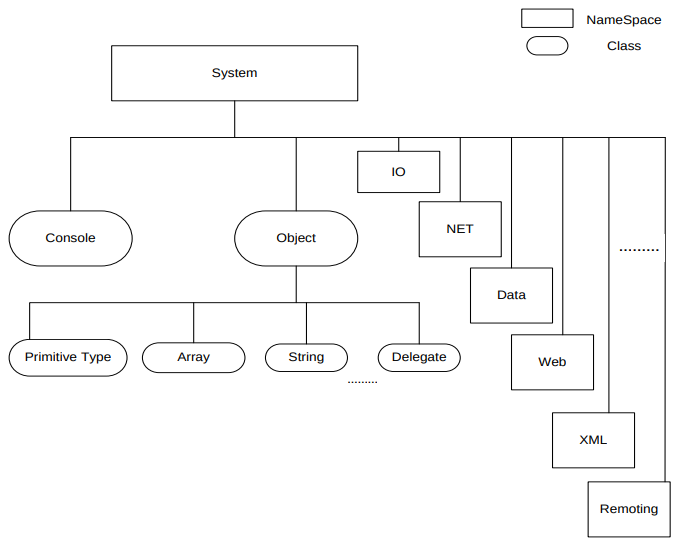
\includegraphics[width=300px]{images/3_Software_Components/.NET_class_library.png}
    \caption{.NET framework class library}
\end{figure}

\subsubsection{Component model of .NET}
The old COM components are replaced by \emph{Assemblies} (or DLL components).
This component technology is unified-language oriented and any component is in the format of pre-compiled MSIL which can be binary plugged in by any other MSIL components or any other .NET compatible clients.
A .NET component is a single pre-compiled and self described CIL module built from one or more classes or multiple modules deployed in a DLL assembly file.

\subsubsection{Assemblies}
Those are the smallest unit of code distribution, deployment and versioning, made of individual components all packaged together.
Those units can be dynamically loaded into the execution engine on demand either from local disk, across network, or even created on-the-fly under program control.

\begin{figure}[H]
    \centering
    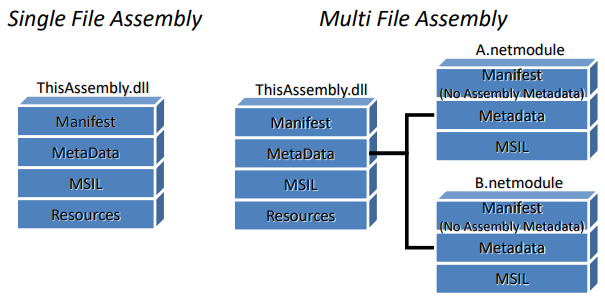
\includegraphics[width=300px]{images/3_Software_Components/assembly_file.png}
    \caption{Assembly file}
\end{figure}

Those units are also:
\begin{itemize}
    \item self-describing: in order to enable data-driven execution;
    \item platform-independent;
    \item bounded by name: we can locate assemblies by querying for its \emph{strong name} made from (publisher token, assembly name, version vector, culture) with version vector made from (major, minor, build, patch);
    \item assembly loading is sensitive to version and policy: programmers and administrators can contribute to policy to assembly-loading behavior;
    \item validated: each time an assembly is loaded, it is subject to a series of checks to ensure the assembly's integrity.
\end{itemize}

The structure of an assembly file is:
\begin{itemize}
    \item Manifest: which is a table of info records such as the one in the strong name, the public key from the publisher, type inference information for the exported types, the list of files inside the archive, information on referenced assemblies reference;
    \item metadata of modules;
    \item CIL code of module;
    \item resources (such as images files).
\end{itemize}

A module has CIL code and metadata but without manifest, thus is not dynamically loadable but it's a building block at compile time in order to build up an assembly module file, and it has the .netmodule extension.

A .dll file is not executable just like a class file while a .exe file, generated by a .NET compiler, has a PE .NET format which is a different version of the PE file (Portable Executable, the standard Microsoft format for executable files) that identifies CLR executable file.

A component can be:
\begin{itemize}
    \item local: can only be accessed locally which means within the same application domain and in the same machine and is .dll;
    \item remote: is a distribute application and can be accessed remotely in the same or different machines. 
\end{itemize}

Moreover a component can be deployed:
\begin{itemize}
    \item as a private component knowing the target client;
    \item as a shared public component: in this case it must be published in a centralized repository: Global Assemby Cache (GAC), typically using its strong name.
    This component supports side-by-side multiple version component execution.
\end{itemize}

.NET component can be composed both via containment or aggregation and even in a mix of both building a flat structure or a nested one.

\subsection{Delegates in CLR and C\#}
A Delegate in CLR and C\# is a type that represents references to methods with a specific parameter list and return type:
\begin{verbatim}
    delegate int MyFun(int i, int j);
\end{verbatim}
for example this is a type with instances holding methods of type \verb|int*int -> int|.
It's similar to function pointers in C/C++ but type-safe and secure.

An instance of a delegate type can hold/refer both to static and to instance methods, of course of the prescribed signature.
The method referred to by a delegate instance can be invoked by passing the list of actual parameters to the instance itself.

Some of the uses for delegates are:
\begin{itemize}
    \item pass methods as arguments to other methods in order to support higher-order functions;
    \item add support for event-based programming using delegates to pass event handlers;
    \item define callback methods.
\end{itemize}
For example:
\begin{verbatim}
class Foo {
    delegate int MyFun(int i, int j);
    static int Add(int i, int j){
        return i + j;
    }
    int Mult(int x, int y){
        return x * y;
    }
    static void Main(string[] args) {
        MyFun fun = new MyFun(Foo.Add);
        Console.WriteLine(fun(2, 3));
        Foo obj = new Foo();
        fun = new MyFun(obj.Mult);
        Console.WriteLine(fun(2, 3));
    }
}
\end{verbatim}

\subsubsection{Closures}
Closures are used in functional programming to close open terms in functions capturing external variables.
Delegates are not equivalent to closures although they are a pair (environment, function) because the environment should be of the same type (class) to which the method belongs.

Can be used in order to introduce elements of functional programming inside C\# for example creating map/filter/reduce variants.

To make event handling in Java the listener must implement an interface in order to specify the method that should be called by the event source to notify.
In C\# instead we can create a delegate object to register the callbacks and then call it in order to notify the listeners.
This approach is more flexible than the Java implementation because:
\begin{itemize}
    \item the management of the subscription and un-subscription is done by the delegate object itself;
    \item the delegate can be hold by a third element which is nor the event source nor any listener, so that list can be use by many sources, so we can implement many-to-many event system;
    \item delegates allow connecting event sources to listeners independent of the types involved because the listener doesn't necessarily needs to implement specific interface;
    \item delegate are by design multicast, so more listener can register their callbacks.
    This one can also be a problem in case we want to build unicast delegates.
\end{itemize}

In order to better support event-based programming using delegate the \verb|event| keyword has been created: if a delegate of a class is labeld with event then outside code will only be able to use \verb|+=| to subscribe and \verb|-=| to un-subscribe.

\subsection{Remoting connectors for .NET Distributed Components}
A remoting channel connections allows a component or a client to access a remote component running in a different application domain in same or different processes.
The \emph{marshaling} makes it possible to invoke a remote method of a distributed component, there are two ways to marsha an object:
\begin{itemize}
    \item MBV: marshal by value in which the server passes a copy of object to the client;
    \item MBR: marshal by reference in which the client creates a proxy of a remote object.
    This is the only choice when a remote component must run at a remote site, and is similar to Java RMI (Remote Method Interface).
\end{itemize}

In the end .NET supports remoting asynchronous callback, based on remoting delegate, this one won't block client while waiting for notification from remote components.
When the client makes a synchronous call to remote method of remote component, it passes a callback method to the server to be called back later through remoting delegate.


